
\section{Kepler and Maxwell vs Pascal}
GM200 and GP100 have both 6GPCs.
Each TPC in Pascal contains 2 SM, in contrast to each TPC corresponding to a single SM in the Kepler and Maxwell architectures
However the number of CUDA Cores per SM keeps decreasing.
The GK110 (Kepler), GM200 (Maxwell), and GP100 (Pascal) have respectively 192, 128 and 64 FP32 CUDA Cores/SM.
The number of SMs per GPU increases faster, giving an increasing amount of CUDA Cores per GPU.
Kepler had a ratio of 1/3 FP64 to FP32 CUDA Cores, which was decreased to 1/32 in Maxwell.
Pascal has increased this ratio back to 1/2.

GK110 and GM200 had a 384-bit GDDR5 memory interface.
GP100 has a 4096-bit memory interface.
3x the bandwidth of the Maxwell GM200 GPU (\textbf{TODO:} How? Is the clock slower? Shouldnt it be > 10x ? (384 vs 4096)).
Can work with larger data sets.

The L2 cache is not much larger with 4096KB, but the total L1 cache available per CUDA Core gets doubled.
The resulting total cache per CUDA Core is thus almost double that of GK110 and GM200.

Kepler implemented atomic memory operations in software just like Fermi in a lock/update/unlock pattern.
Maxwell enabled native hardware support for atomic operations with 32-bit integers and 32-bit and 64-bit compare-and-swap operations.
GP100 allows atomics in Unified Memory, including 32 and 64-bit support for both integers and floats.
\textbf{TODO:} TF/W ?

http://techreport.com/review/30048/exploring-nvidia-pascal-architecture
\begin{itemize}
    % \item Maxwell has only 1/32 FP64 performance
    % \item Pascal has less L2 cache per SM (total 4MB GP100 vs 3MB GM200)
    % \item Pascal has more L1 cache (double per SM: 32,768 $\times$ 32-bit)
    % \item Maxwell was graphics-focused
    % \item GM200 & GP100 have 6 GPCs
    \item FP16 as part of the FP32 ALUs, thus double rate (alike Maxwell Tegra X1 ?)
    \begin{itemize}
        \item GM200 = 6 GPCs $\times$  4SMs $\times$ 4 SIMD 32-wide ALUs
        \item GP100 = 6 GPCs $\times$ 10 SMs (TPCs) $\times$ 2 SIMD 32-wide FP32 ALUs/16-wide FP64 ALUs, with 2 disabled SMs
    \end{itemize}
    % \item HBM2 memory
    \begin{itemize}
        \item 1024-bit memory interface per stack vs 256/512-bit previous
        \item Limited memory per stack (bandwidth linked to capacity)
        \item 4 $\times$ 4 1024-bit stacks of HBM2 $\times$ 8Gb
        \item 700MT/s $\rightarrow$ 720GB/s vs 350GB/s in GDDR5 with 384-bit bus
        \item Requires silicon interposer, which is expensive
        \item NVLink
    \end{itemize}
\end{itemize}


% \begin{figure}[h]%
%  	\begin{center}%
%  		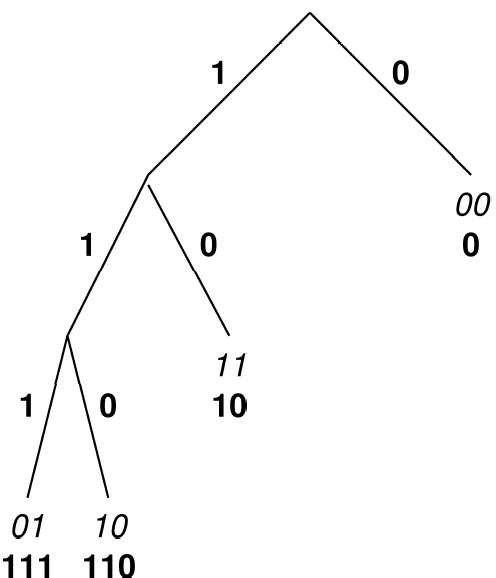
\includegraphics[scale=0.1]{figure1.png}%
%  		\caption{Baum}\label{fig:baum}%
%  	\end{center}%
% \end{figure}
%
% \begin{table}[h]%
%  	\begin{center}%
% 		\caption{Beispieltabelle}\label{tab:example}%
% 	 	\begin{tabular}{c|c}%
%  			Spalte1 & Spalte2\\
%  			\hline
%  			0 & 1\\
%  		\end{tabular}%
%  	\end{center}%
% \end{table}

% % can use a bibliography generated by BibTeX as a .bbl file
% % standard IEEE bibliography style from:
% % http://www.ctan.org/tex-archive/macros/latex/contrib/supported/IEEEtran/bibtex
% \bibliographystyle{IEEEtran}
% % argument is your BibTeX string definitions and bibliography database(s)
% \bibliography{IEEEabrv,references}
